\documentclass[11pt]{article}
\usepackage[margin=1in]{geometry}
\usepackage{amsmath,amssymb,booktabs,tabularx,array,xcolor,graphicx,hyperref}

\hypersetup{
  colorlinks=true,
  linkcolor=blue!55!black,
  citecolor=blue!55!black,
  urlcolor=blue!55!black
}
\newcolumntype{Y}{>{\raggedright\arraybackslash}X}
\newcommand{\microir}{\textsc{micro-ir}}

\title{Reflex Computation:\\
Hard-Arithmetic Scaling and Semantic Execution Blocks}
\author{Working Draft}
\date{August 2026}

\begin{document}
\maketitle

\begin{abstract}
Language models can describe arithmetic procedures while still making exact
execution errors. Conventional tool-use systems address this weakness by
requiring the model to decide to call a calculator and serialize an invocation.
We study bounded local calculator interfaces that act during generation. The
original strict watcher recognizes an arithmetic suffix before an equals sign;
the next iteration adds deterministic LaTeX/Unicode surface normalization and
a lightweight fenced calculator block that executes only when its closing
delimiter arrives. All assisted conditions share the same typed postfix
micro-IR, exact-rational engine, resource bounds, and textual reinjection. A
factorial hard-arithmetic generator crosses four operand widths, four operator
counts, and three structures, while preserving adversarial non-trigger controls
and stage-level traces. A one-checkpoint, one-seed XPU pilot produced
80 generations. On eight arithmetic examples, reflex assistance tied the
unassisted model at 75.0\% exact match, while explicit-tool and oracle
conditions reached 87.5\% and 100\%, respectively. The reflex engine was exact
whenever invoked, but only half of accepted candidates represented the full
intended expression. This small diagnostic run is not a confirmatory result and
does not pass the evidence gate for later mechanisms. The expanded interface is
therefore frozen before an LLM-only adaptive difficulty pilot and a separately
seeded held-out comparison; no expanded-protocol model outcome is claimed yet.
\end{abstract}

\section{Status and Scope}

This document is an implemented next-iteration protocol plus the preliminary
pilot that motivated it, not a completed confirmatory result.
The repository contains a dependency-free calculator/runtime path, deterministic
dataset generation, JSONL traces and summaries, a scripted plumbing check, and
an optional token-by-token Hugging Face adapter. Scripted checks are marked
\texttt{empirical: false}; their expected perfect calculator behavior must not
be cited as model evidence. The XPU pilot reported below is empirical but too
small for model-family, scaling, or replicated performance claims.

Paper 1 asks one question:
\begin{quote}
When a language model naturally exposes a completed arithmetic expression
during generation, does automatic bounded evaluation improve reliability or
cost relative to model-only generation and explicit calculator calls?
\end{quote}

The scope remains calculator only and deterministic syntax interfaces. The
experiment does not test semantic recognition of prose arithmetic, learned routing, persistent
symbolic memory, transactional state, Progressive Retrieval Attention (PRA), or
native key/value access. Those mechanisms would make a positive result harder
to attribute and a negative result harder to diagnose.

\section{Hypotheses}

\paragraph{H1: exact reliability.}
On arithmetic examples for which the strict event is correctly detected and
normalized, reflex assistance increases exact-match accuracy relative to the
same model without assistance.

\paragraph{H2: interface efficiency.}
Reflex or fenced-block assistance reduces model-authored invocation overhead
relative to an explicit calculator condition while remaining competitive in
answer quality and wall time.

\paragraph{H3: difficulty scaling.}
As operator count and operand width increase, reflex accuracy degrades more
slowly than model-only and matched-prompt conditions. The relevant evidence is
the condition-by-difficulty interaction or fitted scaling slope, not one easy
benchmark cell.

\paragraph{H4: model-size leverage.}
Smaller models receive at least as much marginal accuracy benefit from correct
reflex assistance as larger matched-family models. This is tested as a
model-size-by-condition interaction, not inferred from separate unrelated
checkpoints.

These hypotheses are conditional on detection and use. Oracle detection
estimates interface headroom; engine correctness alone does not demonstrate that
the model will expose the syntax or use the inserted result.

\section{Mechanism}

\subsection{Strict generation-time event}

The reflex recognizes an integer arithmetic suffix completed by one equals sign,
for example
\[
\texttt{The total is 37 * 48 =}
\]
and inserts the exact result before later generated text:
\[
\texttt{The total is 37 * 48 = 1776}.
\]
The event is ordinary written arithmetic, not a bespoke API token. Detection is
incremental at character granularity even when a tokenizer supplies multi-character
fragments. Thus, if an equals sign occurs in the middle of a fragment, the result
is inserted before the remainder of that fragment is processed.

The lexical detector accepts digits, whitespace, parentheses, and
\texttt{+}, \texttt{-}, \texttt{*}, \texttt{/}, \texttt{//}, \texttt{\%},
and \texttt{**}. It requires an operator-like symbol, balanced parentheses,
and a digit or closing parenthesis before the equals sign. It suppresses
double-quoted candidates and rejects candidates adjacent to letters,
underscores, or decimal points. Lexical detection remains separate from
normalization: a candidate such as \texttt{+ 2} is logged and then rejected
because it has no binary operation.

\subsection{Typed micro-IR}

The normalizer parses the candidate in expression mode and accepts only integer
constants, binary operations, unary plus, and unary minus. Calls, names,
attributes, indexing, containers, comparisons, booleans, floats, and all other
syntax are rejected. The parsed tree is converted to a canonical postfix
instruction sequence such as
\[
\texttt{PUSH 7; PUSH 5; ADD; PUSH 3; MUL}.
\]
The Python parser is used only to construct and inspect syntax. The source is
never compiled or executed. A separate stack interpreter executes the micro-IR
using exact rational numbers.

\subsection{Resource policy}

Every event is bounded before or during evaluation. The default policy is
shown in Table~\ref{tab:bounds}. Bounds are configuration recorded in each
request, not hidden assumptions.

\begin{table}[t]
\centering
\small
\caption{Default calculator safety and complexity bounds.}
\label{tab:bounds}
\begin{tabularx}{0.82\linewidth}{@{}Yp{0.24\linewidth}@{}}
\toprule
Bound & Default \\
\midrule
Expression characters & 256 \\
AST nodes / depth & 64 / 16 \\
Digits per integer literal & 64 \\
Absolute integer exponent & 12 \\
Numerator or denominator size & 512 bits \\
Stack items & 64 \\
Engine time budget & 25 ms \\
Recognizer suffix buffer & 512 characters \\
\bottomrule
\end{tabularx}
\end{table}

Division by zero, malformed IR, timeout, and resource exhaustion are typed
failures. Failed results are traced but not inserted. Exponent and intermediate
bit limits are checked before a large value can propagate through subsequent
instructions.

\subsection{Observable interrupt pipeline}

Each intervention follows
\[
\textsc{detect}\rightarrow\textsc{normalize}\rightarrow\textsc{route}
\rightarrow\textsc{execute}\rightarrow\textsc{state update}
\rightarrow\textsc{reinject}.
\]
Every transition receives a run ID, sequence number, timestamp, status,
candidate/request IDs, duration where meaningful, and structured details. The
append-only micro-state stores the typed request, result, creation time, detector,
and engine provenance. This is enough to separate detector, parser, engine, and
reinjection failures without importing the later transactional-state design.

\section{Conditions}

All conditions use the same arithmetic examples, checkpoint revision, decoding
budget, and calculator implementation when a calculator is available.

\begin{table}[t]
\centering
\small
\caption{Minimum experimental conditions.}
\label{tab:conditions}
\begin{tabularx}{\linewidth}{@{}p{0.18\linewidth}YY@{}}
\toprule
Condition & Model instruction and capability & Purpose \\
\midrule
LLM only & Return the exact answer; no calculator & Unassisted checkpoint baseline \\
Matched prompt & Work carefully and check operations; no calculator & Stronger prompting without external capability \\
Explicit tool & Model writes \texttt{<tool:calculator>EXPR</tool>} and receives the same engine result & Conventional model-authored invocation baseline \\
Reflex & Model is asked to write the expression followed by one equals sign; runtime detects any valid strict suffix & Proposed automatic condition \\
Normalized reflex & Reflex syntax plus deterministic LaTeX, Unicode, whitespace, and bracket normalization & Surface-robust automatic condition \\
Calculator block & Model writes one fenced calculator block; execution waits for the closing fence & Explicit boundary without an API schema \\
Oracle & Same generation instruction as reflex, but the detector accepts only the gold canonical expression & Detection/selection headroom control \\
\bottomrule
\end{tabularx}
\end{table}

The explicit format is deliberately unambiguous and is not counted as a reflex.
Its parser and the reflex parser converge on the same arithmetic micro-IR and
engine, isolating invocation style from calculator capability. A stronger native
function-calling baseline should be added when the selected model/runtime exposes
a stable function-calling interface; the textual baseline is the portable minimum.

\section{Benchmark}

\subsection{Factorial arithmetic generators}

The legacy deterministic generator crosses operator count with operand digit
width. The separate \texttt{hard\_arithmetic\_v1} generator crosses at least four
operator-count bands, four digit-width bands, and three structures: left chains,
nested trees, and multiplication trees. It includes addition, subtraction,
multiplication, safe exact-rational division, mixed operations, and long
intermediates. Each cell uses identity-derived random seeds, and gold answers are
produced by a separate exact-rational reference evaluator rather than the
calculator implementation under test. The full hard grid contains
\[
4\ \text{operator counts}\times
4\ \text{digit widths}\times
3\ \text{structures}=48\ \text{cells}
\]
before replicate and seed factors. Every generated item is accepted only after
the independent oracle and bounded calculator agree.

This synthetic benchmark isolates scaling and component correctness; it does not
establish ecological prevalence. A later extension may add held-out natural
model traces, but only after freezing annotation rules for whether a generated
prefix contains a valid strict event.

\subsection{Non-trigger and adversarial controls}

Controls include prose containing numbers, ranges, parentheses, quoted
arithmetic, decimal-looking versions, variable equations, and code-like equality.
Additional engine tests cover division by zero, excessive exponents and values,
disallowed calls/names/indexing, and unary-only candidates. Controls are scored
for false intervention and component behavior, not arithmetic answer accuracy.

\subsection{Model and seed sweep}

The primary manifest pins one matched Qwen3 family at 0.6B, 1.7B, and 4B
parameters and uses seeds 17, 29, and 41. Repository commit hashes are stored in
the configuration and copied into run manifests. The model list is an initial
controlled family, not a claim of model-family generality. A second family is
required before making architecture-general claims.

Generation is greedy in the initial adapter so seed variability mainly reflects
future sampled configurations and experimental plumbing; if sampling is enabled,
temperature, top-$p$, and all random states must be pinned. The correctness-first
adapter recomputes the full prefix per generated token after reinjection. This is
intentionally inefficient but semantically transparent. Optimized KV-cache
interception is outside Paper 1 and must not be silently credited to it.

\section{Metrics and Analysis}

\paragraph{End task.}
Report exact rational answer accuracy with 95\% confidence intervals. If a model
states a final answer after receiving a calculator result, score the final claim,
not merely the correct engine value. Report correction, override, and result-use
rates separately.

\paragraph{Components.}
Report intended-expression exposure, candidate recognition, full-expression
selection, normalization acceptance/correctness, engine success/correctness,
reinjection success, result use, and later override separately. Also report
false-intervention rate, intervention count, and state-item count. Oracle
differences localize missed or malformed interface events.

\paragraph{Cost.}
Report prompt, model-generated, and reinjected tokens separately; model calls;
engine and end-to-end wall time; and serialized trace/state growth. Do not present
the correctness-first Hugging Face adapter's full-prefix recomputation as a
production latency estimate.

\paragraph{Scaling and inference.}
Report every operator-count by digit-width cell for each model, condition, and
seed. Estimate condition-by-difficulty and condition-by-model-size interactions,
with paired comparisons because all conditions share examples. Predeclare one
primary endpoint and correct or label exploratory multiple comparisons. Preserve
raw predictions and event traces so component errors can be reclassified.

\section{Frozen Next-Iteration Protocol}

The interface freeze is versioned as
\path{paper1_hard_interfaces_v1}. It retains
\path{strict_arithmetic_v1} unchanged and adds
\path{normalized_arithmetic_v1},
\path{surface_normalizer_v1}, and
\path{calculator_block_v1}. The normalizer maps allowlisted multiplication,
division, Unicode-minus, bracket, and spacing aliases before delegating to the
existing \path{ccpu.arithmetic.postfix.v1} parser. Unknown commands, prose,
variables, quoted arithmetic, and quoted or inline fence examples remain inert.

The block grammar is a line-anchored Markdown-like fence named
\texttt{calculator}. Its contents are collected incrementally, but no candidate
is emitted until the closing fence is complete. Thus a valid intermediate line
cannot execute prematurely. At close, the same surface normalizer and bounded
calculator are used, and a compact typed result is inserted.

The adaptive pilot runs only the LLM-only condition over all 48 cells. Cell
selection uses aggregate exact match to choose regimes near 95\%, 65\%, 30\%,
and 0\%; it never examines assisted outcomes. Once those cells are selected,
their definitions, prompts, grammar, normalizer, and diagnostics remain frozen.
A distinct dataset seed then generates the held-out comparison across all seven
conditions.

Every arithmetic prediction records expression exposure, candidate recognition,
full-expression selection, normalization, execution, reinjection, result use,
and later override independently. Cost records include prompt, generated, and
reinjected tokens, model calls, wall and engine time, serialized trace/state
bytes, and deterministic invocation-delimiter characters. Scripted smoke output
is marked \texttt{empirical: false} and is plumbing evidence only.

\section{Preliminary XPU Pilot}

\subsection{Setup}

We ran a diagnostic pilot with Qwen3-0.6B at pinned revision
\texttt{c1899de} (the full hash is stored in the manifest), PyTorch
2.13.0+XPU, and an Intel integrated GPU. The deterministic sample crossed one
and three operators with one- and two-digit operands, using addition and
multiplication. It contained two examples per cell (eight arithmetic examples)
and eight matched non-trigger controls. One generation seed (17) and five
conditions yielded 80 generations. The 96-token output budget was selected
after a shorter plumbing run exposed truncation; the shorter run is not included
in the results. Confidence intervals are Wilson intervals over only eight
arithmetic observations per condition and are therefore intentionally wide.

\subsection{Results}

\begin{table}[t]
\centering
\small
\caption{Exploratory XPU pilot. Accuracy intervals are 95\% Wilson intervals;
tokens and latency are means. Latency reflects the correctness-first
full-prefix adapter and is not a production estimate.}
\label{tab:xpu-pilot}
\begin{tabular}{@{}lcccc@{}}
\toprule
Condition & Accuracy & Trigger recall & Output tokens & Latency (ms) \\
\midrule
LLM only      & 0.750 [0.409, 0.929] & ---   & 40.56 & 8028 \\
Matched prompt& 0.625 [0.306, 0.863] & ---   & 45.81 & 9380 \\
Explicit tool & 0.875 [0.529, 0.978] & 0.625 & 22.50 & 4410 \\
Reflex        & 0.750 [0.409, 0.929] & 0.750 & 46.06 & 9195 \\
Oracle        & 1.000 [0.676, 1.000] & 1.000 & 15.31 & 2718 \\
\bottomrule
\end{tabular}
\end{table}

The reflex condition did not improve exact-match accuracy over LLM only in this
pilot. Explicit-tool accuracy was numerically higher and oracle intervention was
perfect, but the sample is too small for either difference to support a general
claim. No condition falsely intervened on a control. Accepted explicit-tool
candidates represented the intended expression in every triggered case, whereas
only 50\% of reflex candidates did. Inspection showed that the strict watcher
often intercepted a valid intermediate subexpression rather than the full task
expression. Once a candidate reached the engine, execution correctness was
100\% in both conditions. Reflex result-use was 66.7\%, and one third of used
results were later overridden. These component results locate the present
bottleneck in exposure, selection, and downstream use rather than arithmetic
execution.

\begin{figure}[t]
\centering
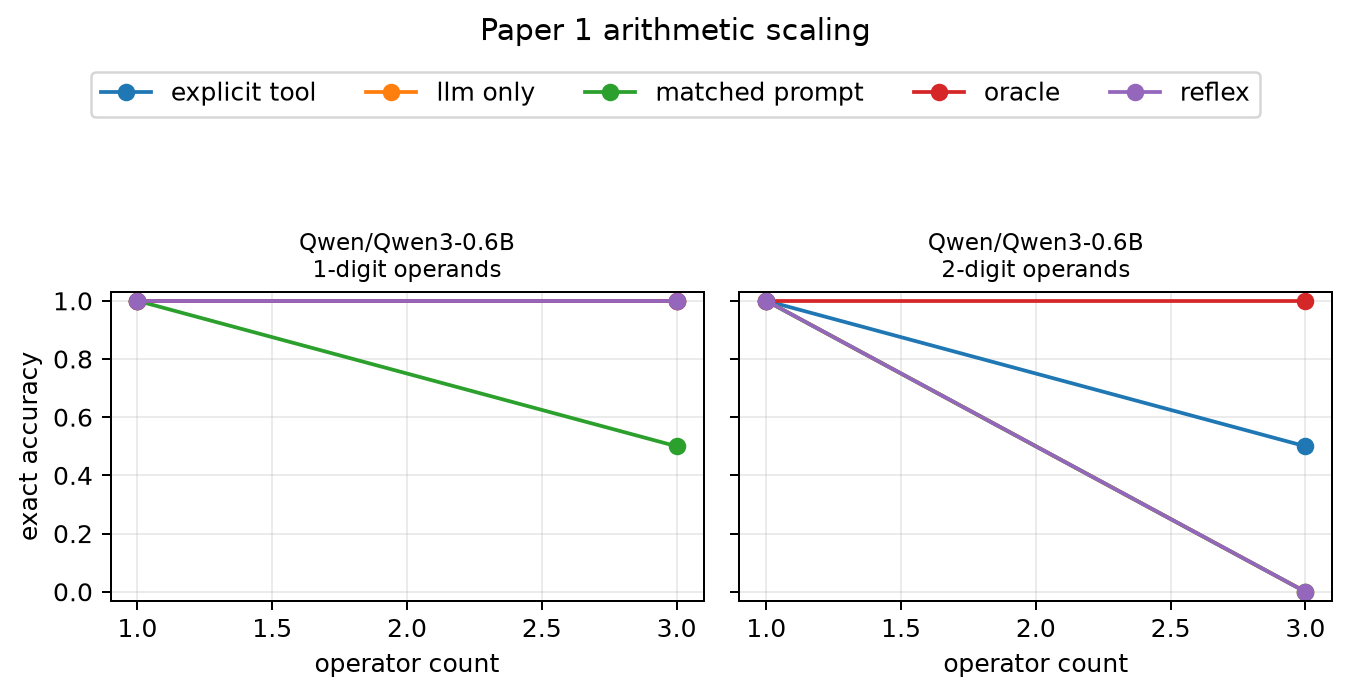
\includegraphics[width=0.94\linewidth]{paper1_xpu_pilot.png}
\caption{Exploratory exact-match accuracy by generated difficulty cell. Each
point contains only two examples; the figure diagnoses plumbing and candidate
behavior and must not be read as a scaling estimate.}
\label{fig:xpu-pilot}
\end{figure}

At this protocol revision H1 is not supported: the automatic reflex tied the
unassisted baseline and failed to dominate explicit invocation. H2--H4 remain
untested because this pilot includes neither a production interface nor the
required model-size and seed sweeps. Paper 2 therefore remains gated. A
confirmatory run must increase examples per cell, use all declared seeds and
model sizes, add a second family, and freeze any detector change before
examining outcomes.

\section{Falsification and Evidence Gate}

The reflex claim is not supported if any of the following holds under matched
capability and declared cost accounting:
\begin{itemize}
  \item answer gains disappear when final model claims, rather than inserted
  engine values, are scored;
  \item false triggers, normalization errors, or ignored results offset exact
  execution gains;
  \item explicit calculator calling matches or dominates the quality--token--latency
  frontier;
  \item reflex and baseline accuracy have indistinguishable difficulty slopes;
  \item gains occur only with oracle detection or only in one easy/model cell; or
  \item results fail to reproduce across seeds or a second model family.
\end{itemize}

Paper 2 is justified only if Paper 1 identifies a reproducible regime where
automatic strict assistance helps and mixed operation types expose a limitation
of one calculator. Paper 3 is not justified by syntax brittleness alone; learned
interrupts require a measured task regime worth extending.

\section{Reproduction}

The reusable runtime lives under \texttt{src/ccpu/common}; Paper 1 code lives
under \texttt{src/ccpu/paper1}. From the repository root, the dependency-free
protocol check is:

\begin{verbatim}
python -m pip install -e .
python -m pytest
python -m ccpu paper1 generate \
  --config configs/paper1/smoke.json \
  --output artifacts/paper1/smoke/dataset.jsonl
python -m ccpu paper1 validate \
  --dataset artifacts/paper1/smoke/dataset.jsonl
python -m ccpu paper1 simulate \
  --dataset artifacts/paper1/smoke/dataset.jsonl \
  --output-dir artifacts/paper1/smoke/run
\end{verbatim}

The pinned pretrained path is:

\begin{verbatim}
python -m pip install -e ".[hf]"
python -m ccpu paper1 generate \
  --config configs/paper1/primary.json \
  --output artifacts/paper1/primary/dataset.jsonl
python -m ccpu paper1 run-hf \
  --dataset artifacts/paper1/primary/dataset.jsonl \
  --config configs/paper1/primary.json \
  --output-dir artifacts/paper1/primary/run
\end{verbatim}

The reported XPU pilot uses the direct interpreter from the validated XPU
environment and can be reproduced with:

\begin{verbatim}
$py = 'C:\Users\j.simao\.venvs\modal-llm-xpu\Scripts\python.exe'
$env:PYTHONPATH = (Resolve-Path src).Path
& $py -m ccpu paper1 generate \
  --config configs/paper1/xpu_pilot.json \
  --output artifacts/paper1/xpu_pilot/dataset.jsonl
& $py -m ccpu paper1 run-hf \
  --dataset artifacts/paper1/xpu_pilot/dataset.jsonl \
  --config configs/paper1/xpu_pilot.json \
  --output-dir artifacts/paper1/xpu_pilot/run96
& $py -m ccpu paper1 replay \
  --dataset artifacts/paper1/xpu_pilot/dataset.jsonl \
  --completions artifacts/paper1/xpu_pilot/run96/predictions.jsonl \
  --output-dir artifacts/paper1/xpu_pilot/final
\end{verbatim}

Device selection for \texttt{device: auto} is CUDA, then XPU, then CPU. The
replay step applies the current frozen evaluator to preserved generations and
records both the source prediction hash and rescore provenance.

Use \texttt{--limit}, \texttt{--model}, and repeated \texttt{--condition}
arguments for resource preflight. Each run writes predictions, full traces,
summary tables, hashes, configuration, model metadata, environment information,
and git revision/dirty status. The replay command permits model generation in a
separate harness while preserving identical controller and evaluation semantics.
The \texttt{plot} command renders the machine-readable scaling cells as accuracy
curves by model, operand width, condition, and operator count.

\section{Limitations}

The elicitation instruction asks reflex models to expose an expression followed
by an equals sign. This is less explicit than an API call but still changes
generation behavior, and a model that answers directly may never trigger. Both
trigger rate and conditional-on-trigger accuracy are therefore necessary. The
strict lexical grammar does not understand intent and will miss prose arithmetic;
expanding semantics belongs to Paper 3. Quote suppression is deliberately
limited, and code-like or unusual formatting remains an adversarial surface.

The synthetic task controls arithmetic complexity but not realistic discourse.
The textual explicit-tool baseline may understate a model's native structured
function-calling ability. Full-prefix token recomputation overstates runtime
cost. The preliminary XPU run has one checkpoint, one seed, and eight arithmetic
examples, so its intervals, cell curves, and condition ordering are unstable.
Finally, exact calculator output cannot repair an incorrectly copied
expression, a model that ignores the result, or a task whose premises are wrong.

\section{Related Work}

Toolformer trains language models to decide when and how to invoke APIs,
including a calculator \cite{toolformer}. PAL delegates model-generated programs
to an interpreter \cite{pal}, while ReAct interleaves model-authored reasoning and
actions \cite{react}. These systems establish the value of external execution.
Paper 1 isolates a different control point: a runtime recognizes ordinary strict
arithmetic already emerging in the output and invokes a bounded engine without a
function-name decision. The comparison to explicit invocation is empirical; the
paper does not assume that the reflex interface is better.

\section{Conclusion}

Paper 1 reduces the cognitive-coprocessor proposal to its smallest credible
experiment. A character-incremental detector, typed allowlisted micro-IR, exact
bounded calculator, append-only state, and immediate text reinjection are enough
to test whether automatic computation can improve an autoregressive stream.
The implementation is complete at protocol level, and the first XPU pilot
demonstrates end-to-end generation, intervention, replay, and component scoring.
It does not show an automatic-assistance gain: reflex accuracy tied LLM only,
while candidate selection and result use remained imperfect. Model sweeps and
replicated analysis remain required before any positive or negative architecture
claim, and the Paper 2 evidence gate remains closed.

\begin{thebibliography}{9}

\bibitem{toolformer}
T.~Schick, J.~Dwivedi-Yu, R.~Dessi, R.~Raileanu, M.~Lomeli, L.~Zettlemoyer,
N.~Cancedda, and T.~Scialom.
Toolformer: Language models can teach themselves to use tools.
\emph{NeurIPS}, 2023.
\url{https://arxiv.org/abs/2302.04761}.

\bibitem{pal}
L.~Gao, A.~Madaan, S.~Zhou, U.~Alon, P.~Liu, Y.~Yang, J.~Callan, and G.~Neubig.
PAL: Program-aided language models.
\emph{ICML}, 2023.
\url{https://arxiv.org/abs/2211.10435}.

\bibitem{react}
S.~Yao, J.~Zhao, D.~Yu, N.~Du, I.~Shafran, K.~Narasimhan, and Y.~Cao.
ReAct: Synergizing reasoning and acting in language models.
\emph{ICLR}, 2023.
\url{https://arxiv.org/abs/2210.03629}.

\end{thebibliography}

\end{document}
